\documentclass{article}
\usepackage[margin=0.75in]{geometry}
\usepackage{graphicx} % For including images
\usepackage{hyperref} % For clickable references

\begin{document}

\begin{figure}
    \centering
    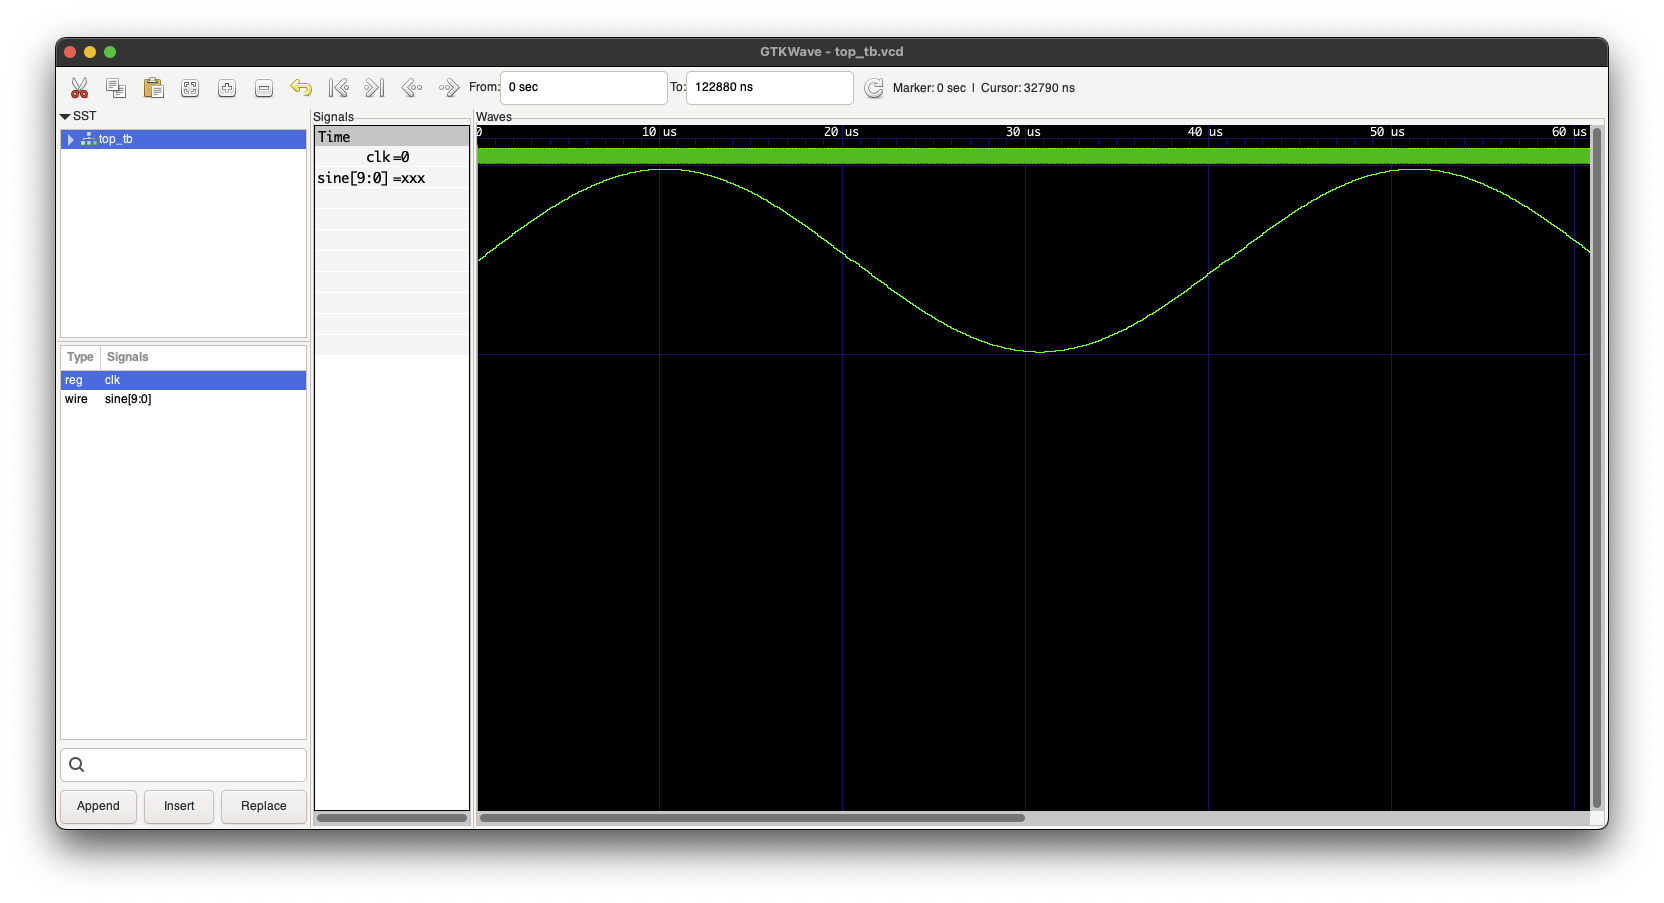
\includegraphics[width=1\textwidth]{sim.png}
    \caption{Simulation output of the sine wave generator circuit.}
    \label{fig:simulation}
\end{figure}

\begin{figure}
    \centering
    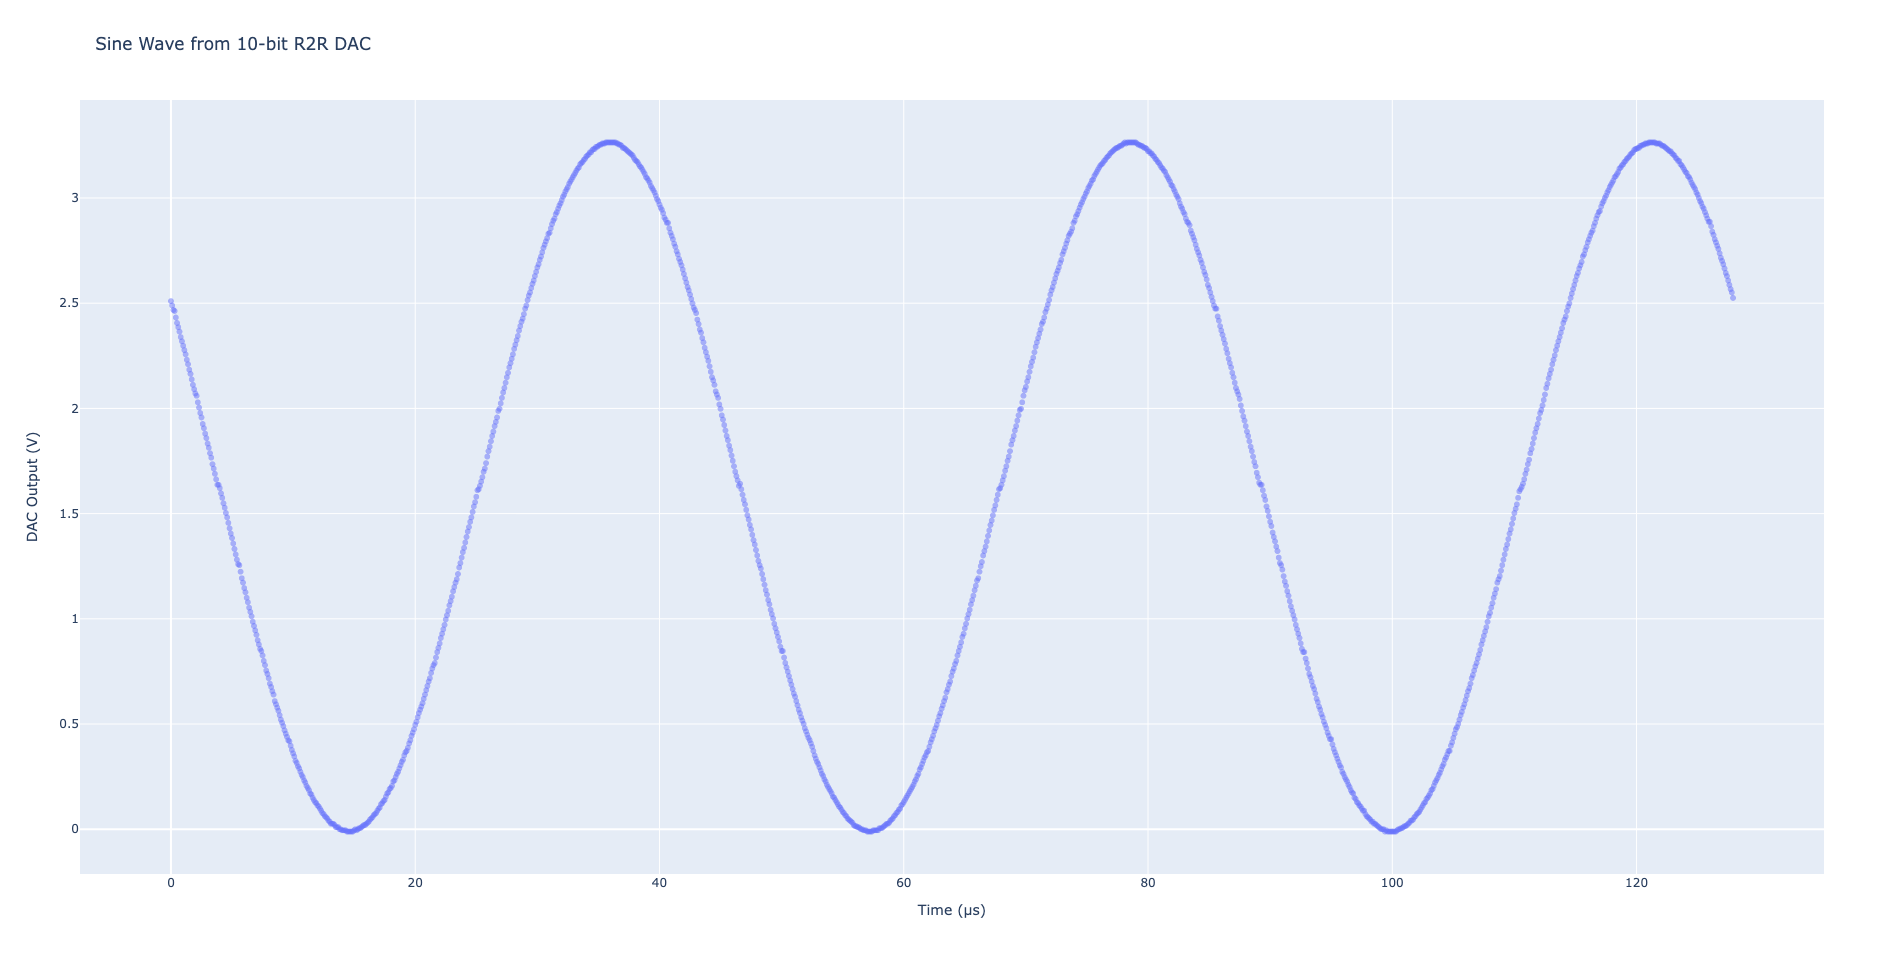
\includegraphics[width=1\textwidth]{plot.png}
    \caption{Oscilloscope capture of the DAC output.}
    \label{fig:oscilloscope}
\end{figure}

\clearpage

The circuit comprises a memory unit that reads from prestored values for the first quarter of a sine wave period. Since a sine function is periodic and symmetric, only 128 9-bit values are needed to generate 512 10-bit samples of a full sine wave. 

For DAC output centered at 1.66V (half of 3.3V), the values from memory are shifted up by 512. For the first quarter, this is sufficient. For the second, third, and fourth quarters, the values are mirrored, negated, and mirrored and negated before being shifted, respectively, for each quarter. Each bit of the read value is then connected to D0-D9 of the R-2R ladder DAC.

The output of the testbench (see Figure \ref{fig:simulation}) and the analog oscilloscope (see Figure \ref{fig:oscilloscope}) are plotted in the figures above.

\end{document}
